%-------------------------
% Resume in Latex
% Author : Andrei Shestakov
% License : MIT
%------------------------

\documentclass[letterpaper,11pt]{article}

\usepackage{latexsym}
\usepackage[empty]{fullpage}
\usepackage{titlesec}
\usepackage{marvosym}
\usepackage[usenames,dvipsnames]{color}
\usepackage{verbatim}
\usepackage{enumitem}
\usepackage[pdftex]{hyperref}
\usepackage{fancyhdr}
\usepackage{graphicx}

\graphicspath{{pictures/}}

\pagestyle{fancy}
\fancyhf{} % clear all header and footer fields
\fancyfoot{}
\renewcommand{\headrulewidth}{0pt}
\renewcommand{\footrulewidth}{0pt}

% Adjust margins
\addtolength{\oddsidemargin}{-0.375in}
\addtolength{\evensidemargin}{-0.375in}
\addtolength{\textwidth}{1in}
\addtolength{\topmargin}{-.5in}
\addtolength{\textheight}{1.0in}

\urlstyle{same}

\raggedbottom
\raggedright
\setlength{\tabcolsep}{0in}

% Sections formatting
\titleformat{\section}{
  \vspace{-4pt}\scshape\raggedright\large
}{}{0em}{}[\color{black}\titlerule \vspace{-5pt}]

%-------------------------
% Custom commands
\newcommand{\resumeItem}[2]{
  \item\small{
    \textbf{#1}{. #2 \vspace{-2pt}}
  }
}

\newcommand{\resumeSubheading}[4]{
  \vspace{-1pt}\item
    \begin{tabular*}{0.97\textwidth}{l@{\extracolsep{\fill}}r}
      \textbf{#1} & #2 \\
      \textit{\small#3} & \textit{\small #4} \\
    \end{tabular*}\vspace{-5pt}
}

\newcommand{\resumeSubItem}[2]{\resumeItem{#1}{#2}\vspace{-4pt}}

\renewcommand{\labelitemii}{$\circ$}

\newcommand{\resumeSubHeadingListStart}{\begin{itemize}[leftmargin=*]}
\newcommand{\resumeSubHeadingListEnd}{\end{itemize}}
\newcommand{\resumeItemListStart}{\begin{itemize}}
\newcommand{\resumeItemListEnd}{\end{itemize}\vspace{-5pt}}

%-------------------------------------------
%%%%%%  CV STARTS HERE  %%%%%%%%%%%%%%%%%%%%%%%%%%%%


\begin{document}

%----------HEADING-----------------
\begin{tabular*}{\textwidth}{l@{\extracolsep{\fill}}r}
  \textbf{\href{http://ornicum.ru/}{\Large Andrei Shestakov}} \\
  DOB: July 10 1984 & Marital status : Single \\
  Email : \href{mailto:ornicum@gmail.com}{ornicum@gmail.com} & Mobile (Russian Federation) : +7-961-610-9035 \\
  Skype id : ornicum & LinkedIn: \href{https://www.linkedin.com/in/andrey-shestakov-4450b24}{Andrey Shestakov} \\
\end{tabular*}

  I have also Telegram, WhatsApp and Viber on russian mobile phone.


%-------------ABOUT-------------------
\section{About}

\begin{figure}[h!]
  \begin{minipage}[h!]{.2\textwidth}
    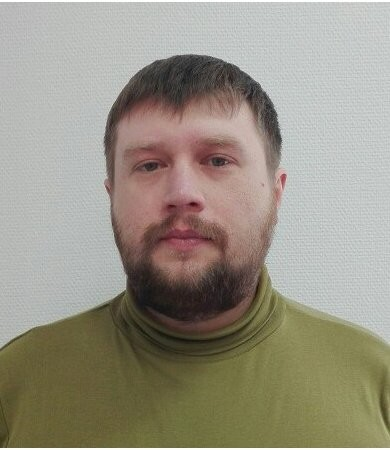
\includegraphics[scale=0.25]{AndreiShestakov0.png}
  \end{minipage}
  \hfil
  \begin{minipage}[h!]{0.8\textwidth}

Hi, I'm Andrei. I'm from Russia, Siberia.

Now I'm living in Antalya, Turkey.

Since 2007 I've been working in commercial software development. I have worked in different scaled projects. From little desktop applications to industrial solutions.

My strong points are responsibility and quality. You will get bad job from me never. I'm sure that any project must work and must be done carefully on every stage. Also you will lose me never. Usually I warn in advance if I need be absent and be offline long time.

My English is good for chat and email. Let me a chance for more verbal skills practices and our conversation will be on best level.
  \end{minipage}
\end{figure}

I have a Bachelors in Applied Mathematics and Computer Science from Novosibirsk State Technical University, in Russia. Also my diploma passed nostrification in Czech Technical University in Prague and got education level on Master degree. My specialization is statistics.

I like my profession and I will glad to work using my knowledge in algorithms, statistics, complex computing and so on. I have wide experience in commercial software engineering for realizing your complex algorithmic computing project on best level.

I'm developing primarily on C/C++ and Python (versions 2.5.x+ and 3.5+).


%-----------OBJECTIVE-----------------
\section{Objective}
  \begin{itemize}
    \item Senior Python Developer
    \item Team Lead
    \item System Architect
    \item Middle C++ Developer
  \end{itemize}


%-------PROGRAMMING SKILLS------------
\section{Programming Skills}
  
  \begin{figure}[h!]
    \begin{minipage}[h!]{0.49\textwidth}
      \begin{itemize}
        \item {OOP/OOD}
          \begin{itemize}
            \item OOP is main instrument for C++ and Python, design patterns need to know for good architecture and I know it.
          \end{itemize}
        \item{C/C++}
          \begin{itemize}
	    \item STL (exclude last standards since C++14, I'm not so good in it)
	    \item POSIX
	    \item multithreading
	    \item multiprocessing
	    \item Qt 4.x.x+
          \end{itemize}
      \end{itemize}
    \end{minipage}
    \hfill
    \begin{minipage}[h!]{0.49\textwidth}
      \begin{itemize}
        \item{SQL}
          \begin{itemize}
            \item MySQL
	    \item PostgreSQL
         \end{itemize}
        \item{NoSQL}
          \begin{itemize}
            \item Redis
	    \item Cassandra
          \end{itemize}
        \item{Administration}
          \begin{itemize}
            \item I have wide experience in administration UNIX-based operation systems since 2003.
          \end{itemize}
      \end{itemize}
    \end{minipage}
  \end{figure}
  \begin{figure}[h!]
    \begin{minipage}[h!]{0.49\textwidth}
      \begin{itemize}
      \item{Python}
        \begin{itemize}
	  \item STL
          \item Scrapy
          \item Django
	  \item Flask
        \end{itemize}
      \end{itemize}
    \end{minipage}
    \begin{minipage}[h!]{0.49\textwidth}
      \begin{itemize}
        \item{}
          \begin{itemize}
	    \item Tornado
            \item Cherrypy
            \item Sqlalchemy
            \item asyncio (include aiohttp, aioredis and so on)
          \end{itemize}
      \end{itemize}
    \end{minipage}
  \end{figure}    

%-----------EDUCATION-----------------
\section{Education}
  \resumeSubHeadingListStart
    \resumeSubheading
      {Novosibirsk State Technical University}{Novosibirsk, Russia}
      {Bachelor of Applied Mathematics and Computer Science (Statistics); GPA: 4.32 / 5.00 } {Sep. 2002 -- June. 2007}
  \resumeSubHeadingListEnd


%-----------EXPERIENCE-----------------
\section{Experience}
  \resumeSubHeadingListStart

    \resumeSubheading
      {DataArt}{Saint Petersburg, Russia}
      {Senior Software Engineer}{July 2021 - March 2023}
      \resumeItemListStart
        \resumeItem{Description}
	  {DataArt is greate outstaff company with fintech specialization. Main markets are USA and Europe. The project I've been working for was connected with driver insurance in UK.}
	\resumeItem{Role}
	  {The main goal of our team was splitting monolith legacy project to microservices and adding integration with a new mobile application.}
	\resumeItem{Technologies}
	  {AWS, docker, Python 3, Django, FastAPI, PostgreSQL, gRPC, microservices}
      \resumeItemListEnd

    \resumeSubheading
      {Demigos}{Remote}
      {Senior Software Engineer}{August 2020 - July 2021}
      \resumeItemListStart
        \resumeItem{Description}
	  {Demigos is a small outsourcing company in Ukraine. In general they work on US market.}
	\resumeItem{Role}
	  {I led backend part of project for US(CA) Realty.}
	\resumeItem{Technologies}
	  {AWS, docker, Python 3, Django, Celery, PostgreSQL, GraphQL, Redis}
      \resumeItemListEnd

    \resumeSubheading
      {SK Hynix Memory Solutions Eastern Europe}{Minsk, Belarus}
      {Senior Software Engineer}{May 2018 - June 2020}
      \resumeItemListStart
	\resumeItem{Description}
	 {SK Hynix R\&D center in Minsk is specialized in SSD development. There are several departments: SSD Hardware Verification, Advanced Algorithms, Firmware, Tools, Hardware Simulator and Software Quality Engineering.

	SK Hynix has several SSD projects per year. It can be SATA or NVMe projects also the projects at the same time can be Client or Enterprise. Enterprise SSD has some capacitors that help to save cached data to NAND in 15 microseconds.}
	\resumeItem{Role}
	{I was working in SQE team and led project for testing Vendor Specific Commands (it's command set for different Vendor Specific Tools for SSD). My main task was not writing tests for Vendor Specific Commands only, but also creating arcitecture and infrastructure for making all Vendor Specific Command tests common, if it was possible.}
        \resumeItem{Technologies}
          {Python 2.7 and internal framework, C and C++ code debug.}
      \resumeItemListEnd


    \resumeSubheading
      {Freelance}{Russia}
      {Software Engineer}{2009 - Present}
      \resumeItemListStart
        \resumeItem{Description}
          {There were many different projects.

           There are biggest and most interesting.
	   \begin{enumerate}
             \item System for scraping, collecting and analysing data from bookmaker's sites. It was written on Django.
             \item System for collection data from sport exchange betfair.com and also tools for statistical analysis. It was system with complex architecture that using server software written on C++, PostgreSQL as database, Redis for collecting bad structured data, Tornado as web-part server, web-sockets.
             \item Web currency exchanger. Also in this project I wrote begin part of internet banking.
	   \end{enumerate}}
        \resumeItem{Role}
          {System Administrator, C++ Software Engineer, Python Software Engineer.}
      \resumeItemListEnd

    \resumeSubheading
      {Mobalytics}{Saint Petersburg, Russia}
      {Senior Software Engineer}{Oct 2016 - Sep 2017}
      \resumeItemListStart
        \resumeItem{Description}
          {It's a startup for competiteve e-sports gamers like online coucher. There were several projects: know-how as GPI (General Performance Index), pre-game, post-game and statistics.}
	\resumeItem{Role}
	  {I led project named "Statistics" that shows different statistic characteristics of player for matches, seasons, characters and so on.}
        \resumeItem{Technogies}
	  {We changed technologies stack 5 times per year. Started from Python 2.7, Django, PostgreSQL, Celery, RabbitMQ and ended on Python 3.6, Cassandra, asyncio, Microservices, Kubernetes}
      \resumeItemListEnd

     \resumeSubheading
       {Loveplanet LLC}{Saint Petersburg, Russia}
       {C/Python Developer}{Jun 2016 - Oct 2016}
       \resumeItemListStart
         \resumeItem{Description}
	   {Dating service with backend written as module for Apache 1.2 and tuned MySQL as database.}
	 \resumeItem{Role}
	   {My main task was creating anomaly traffic detection system. I used R-library by Twitter.}
	 \resumeItem{Technologies}
	   {C, Python, R, MySQL}
       \resumeItemListEnd

     \resumeSubheading
       {BARS Group}{Kazan and Saint Petersburg, Russia}
       {Middle Python Developer}{Dec 2015 - May 2016}
       \resumeItemListStart
         \resumeItem{Description}
	   {Company is part of RosTech, specialized on developing cloud Case/Buisness/Workflow management services for Russian Government.}
	 \resumeItem{Role}
	   {Developing cloud service named "Staff and salary", main client at that moment was Federal Treasury of Russian Federation.}
	 \resumeItem{Technologies}
	   {Python 2.7, Django-like internal framework, PostgreSQL, ExtJS.}
       \resumeItemListEnd

     \resumeSubheading
       {GDS Ltd}{Novosibirsk, Russia}
       {Software Engineer}{Apr 2013 - Jan 2014}
       \resumeItemListStart
         \resumeItem{Description}
	   {It's a small outsource company where founder is my friend. He asked me to work for a project for Logistics in Military Aircraft from scratch. And we did our work good. The first part of the system was worked well, it was full-fledged prototype. But the other parts did another company.}
	 \resumeItem{Role}
	   {Architecture of 3 server and 2 client solutions. Also developing network interfaces, GUI and so on.}
	 \resumeItem{Technologies}
	   {C++, Qt 4.6.+, PostgreSQL}
       \resumeItemListEnd

     \resumeSubheading
       {AcademSoft}{Novosibirsk, Russia}
       {Junior Software Developer}{Jul 2010 - Apr 2011}
       \resumeItemListStart
         \resumeItem{Description}
	   {The company has 2 projects: billing and popular automobile navigator in Russia. I worked in the last one.}
	 \resumeItem{Role}
	   {I had a small project on Qt for PC, updater for "Navitel navigator" on mobile platforms. Also I worked in Porting Department, so I had tasks for debugging troubles with porting software to different platforms.}
	 \resumeItem{Technologies}
	   {C++, Qt 4.5.+}
       \resumeItemListEnd

     \resumeSubheading
       {Externet Group}{Novosibirsk, Russia}
       {Software Developer}{Aug 2008 - Feb 2009}
       \resumeItemListStart
         \resumeItem{Description}
	   {VoIP service for buisness.}
	 \resumeItem{Role}
	   {Main tasks.
	     \begin{enumerate}
               \item Developing and support server software (VoIP).
               \item Configuring and support Asterisk server.
	       \item New hardware researching (VoIP gateways).
	       \item Writing documentation.
             \end{enumerate}
	   }
	 \resumeItem{Technologies}
	   {C++, VoIP, SIP, Asterisk server}
       \resumeItemListEnd

     \resumeSubheading
      {EMA ltd}{Novosibirsk, Russia}
      {Software Engineer} {Jul 2007 - Aug 2008}
      \resumeItemListStart
        \resumeItem{Description}
          {Automation in Energetics. Company had 14 server and several client solutions for different tasks on power plants.}
        \resumeItem{Role}
          {My main tasks.
            \begin{enumerate}
	      \item Migration system calls library from OS iRMX to Linux.
              \item Developing and support server software.
              \item Developing architecture of separate parts of software.
              \item Writing documentation.
            \end{enumerate}
          }
        \resumeItem{Technologies}
          {C, Oracle}
      \resumeItemListEnd

  \resumeSubHeadingListEnd


%-----------SPECIAL SKILLS-----------
\section{Special Skills}
  \begin{itemize}
    \item Native Russian.
    \item Intermediate English.
    \item Skipper license by ISSA.
    \item Hobbies: playing guitar, mountaineering, fishing.
  \end{itemize}

%-------------------------------------------
\end{document}

